\newpage
\section{Numerical Results}
The aim of the numerical results is \textcolor{red}{What do I actually want to achieve with this?}\newline
\textcolor{red}{Should I make a subsection for the parameter determination or should I just put that into the appendix? $\rightarrow$ appendix, but state here} \newline
\textcolor{red}{Should I talk about run time and boundary conditions again?}

\subsection{Validation}
add graphs that show expected behavior of triplet-gap: zero-energy edge states, second gap in bulk \newline
show influence of SOC on gap (singlet and triplet) as well as influence of RKKY\newline
decide which graphs are better suited: gap or LDOS? \newline
show which parameter ranges allows for self-consistency (because it converges) and their physical significance \newline
$\gamma$ enhances the influence of the RKKY interaction on the gap \textcolor{red}{WHY?} \newline

In figure \ref{fig:relative_gap}, the relative gap calculated based on $\Delta_s - \Delta_t$ is calculated.
It shows that for $V=0.3$ the triplet gap is higher in magnitude than the singlet gap.
The results for $V \geq 0.4$ did not converge in the self-consistency approach.
A comparison with the LDOS fulfills the expectation based on Section \ref{sec:andreev} that only for $\Delta_t > \Delta_s$ there exist zero-energy states.
Figure \ref{fig:ldos_gap_andreev} shows this directly.

\begin{figure}[h!]
    \centering
    \includegraphics[width=0.95\textwidth]{Images/gap_relative_20x20_U2.0_J0_gamma0.2.png}
    \caption{The relative gap calculated based on $\Delta_s - \Delta_t$. The results for $V \geq 0.4$ did not converge, but for $V=0.3$ the triplet gap is larger in magnitude than the singlet gap.}
    \label{fig:relative_gap}
\end{figure}

\begin{figure}[H]
    \centering
    \label{fig:ldos_gap_andreev}
    \subfigure[LDOS]{\includegraphics[width=0.48\textwidth]{Images/ldos_10_12_0.5_2.0_0.5_0.2_0_1_5.png}}
    \subfigure[gap]{\includegraphics[width=0.48\textwidth]{Images/gap_10_12_0.5_2.0_0.5_0.2_0_1_5.png}}
    \caption{LDOS and gap in direct comparison. There only exist zero-energy states where the triplet gap is larger than the singlet gap.}
\end{figure}

The triplet gap $\Delta_t$ is determined by the expectation value $\langle c_i c_{i\pm1}\rangle$, where the calculations for $\pm 1$ have to be done separately.
In figure \ref{fig:triplet_leftright}, the two different self-consistent calculations are compared to each other. 
Since the edge values have to be fixed manually, the two approaches differ on the edges, but are identically in the bulk.

\begin{figure}[h!]
    \centering
    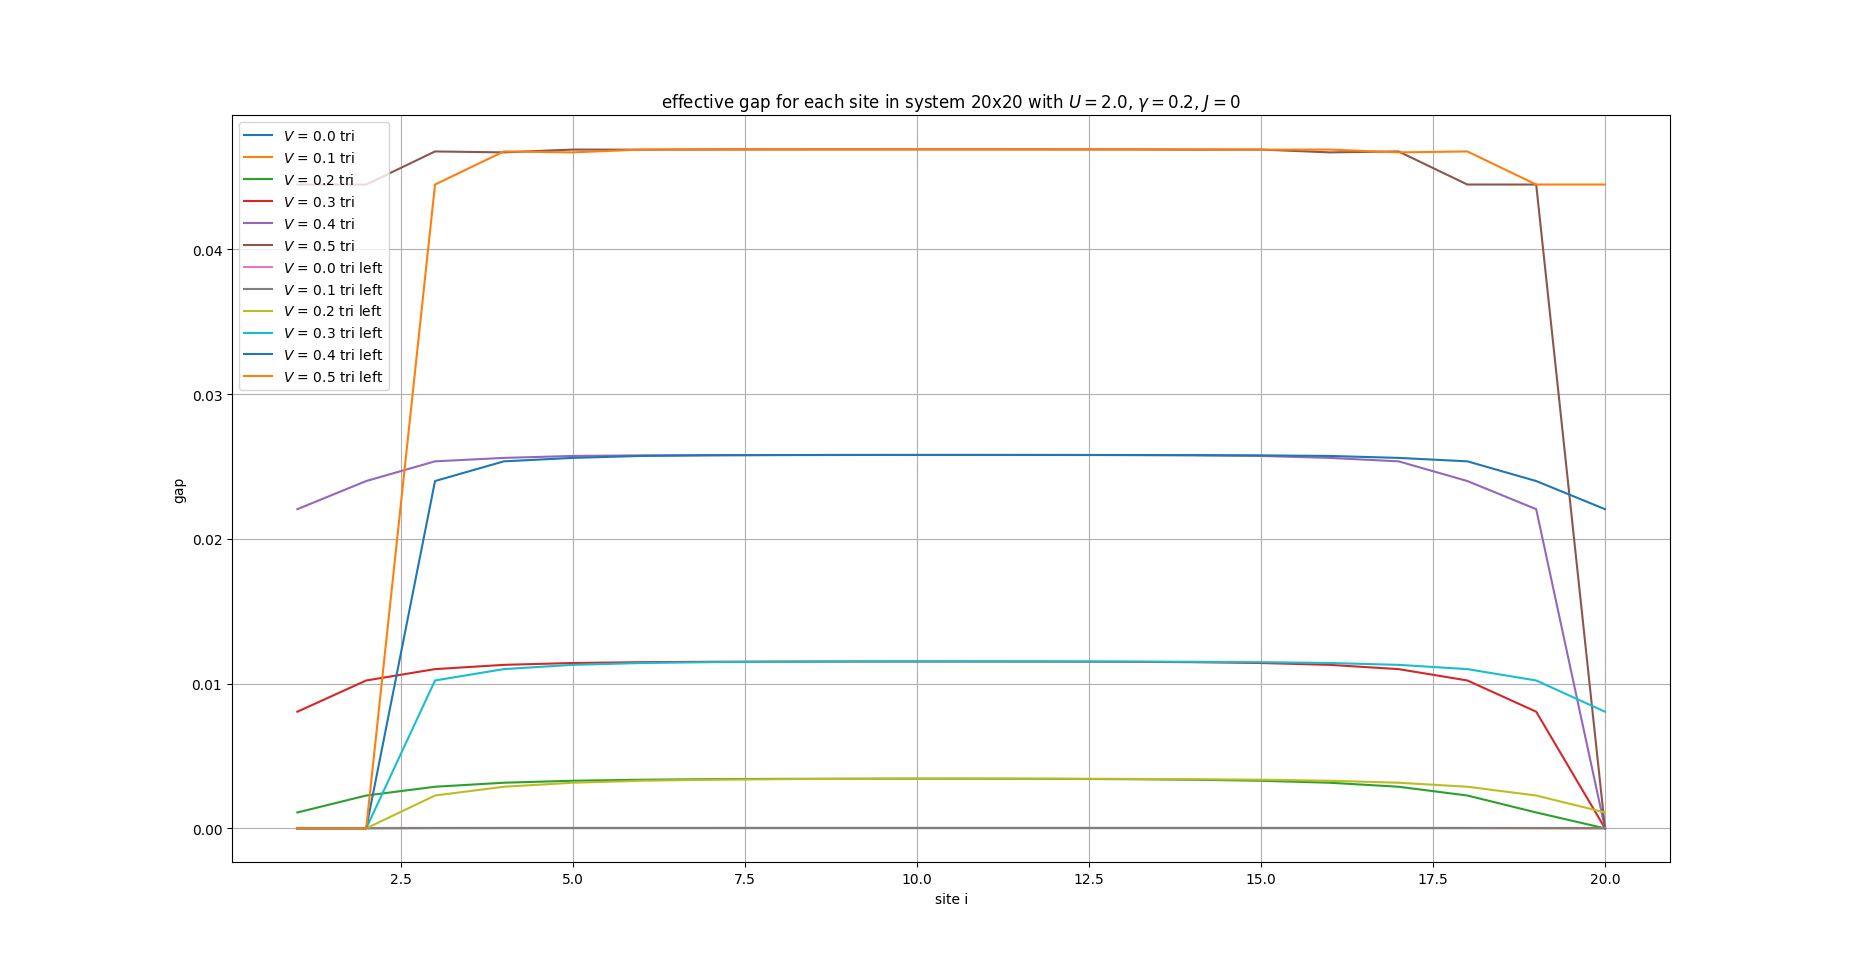
\includegraphics[width=0.95\textwidth]{Images/33_leftright_comp_20x20.png}
    \caption{The triplet gap calculated based on $\langle c_i c_{i+ 1}\rangle$ (tri) and $\langle c_i c_{i-1}\rangle$ (tri left). The edges differ because of the manually fixed values, but the bulk gaps are identical.}
    \label{fig:triplet_leftright}
\end{figure}

The influence of the RKKY interaction onto the gap structure is of high interest in this work.
Figure \ref{fig:ldos_triplet_rkky} shows that the LDOS at the site of an impurity spin is altered such by the RKKY that for weak SOC the RKKY interaction enhances the triplet gap structure, but for strong SOC it weakens the exact same structure. \newline
The damping of the triplet gap peaks in the LDOS due to RKKY interaction gets stronger with stronger RKKY as can be seen in Figure \ref{fig:ldos_rkky_stronger}.

\begin{figure}[H]
    \centering
    \subfigure[LDOS without RKKY]{\includegraphics[width=0.48\textwidth]{Images/gamma_35x35_ldos_V0.1.png}}
    \subfigure[LDOS with $R=1.5$, impurities at 1 ad 17]{\includegraphics[width=0.48\textwidth]{Images/gamma_35x35_ldos_V0.1_R1.5.png}}
    \caption{LDOS and gap in direct comparison. There only exist zero-energy states where the triplet gap is larger than the singlet gap.}
    \label{fig:ldos_triplet_rkky}
\end{figure}

\begin{figure}[H]
    \centering
    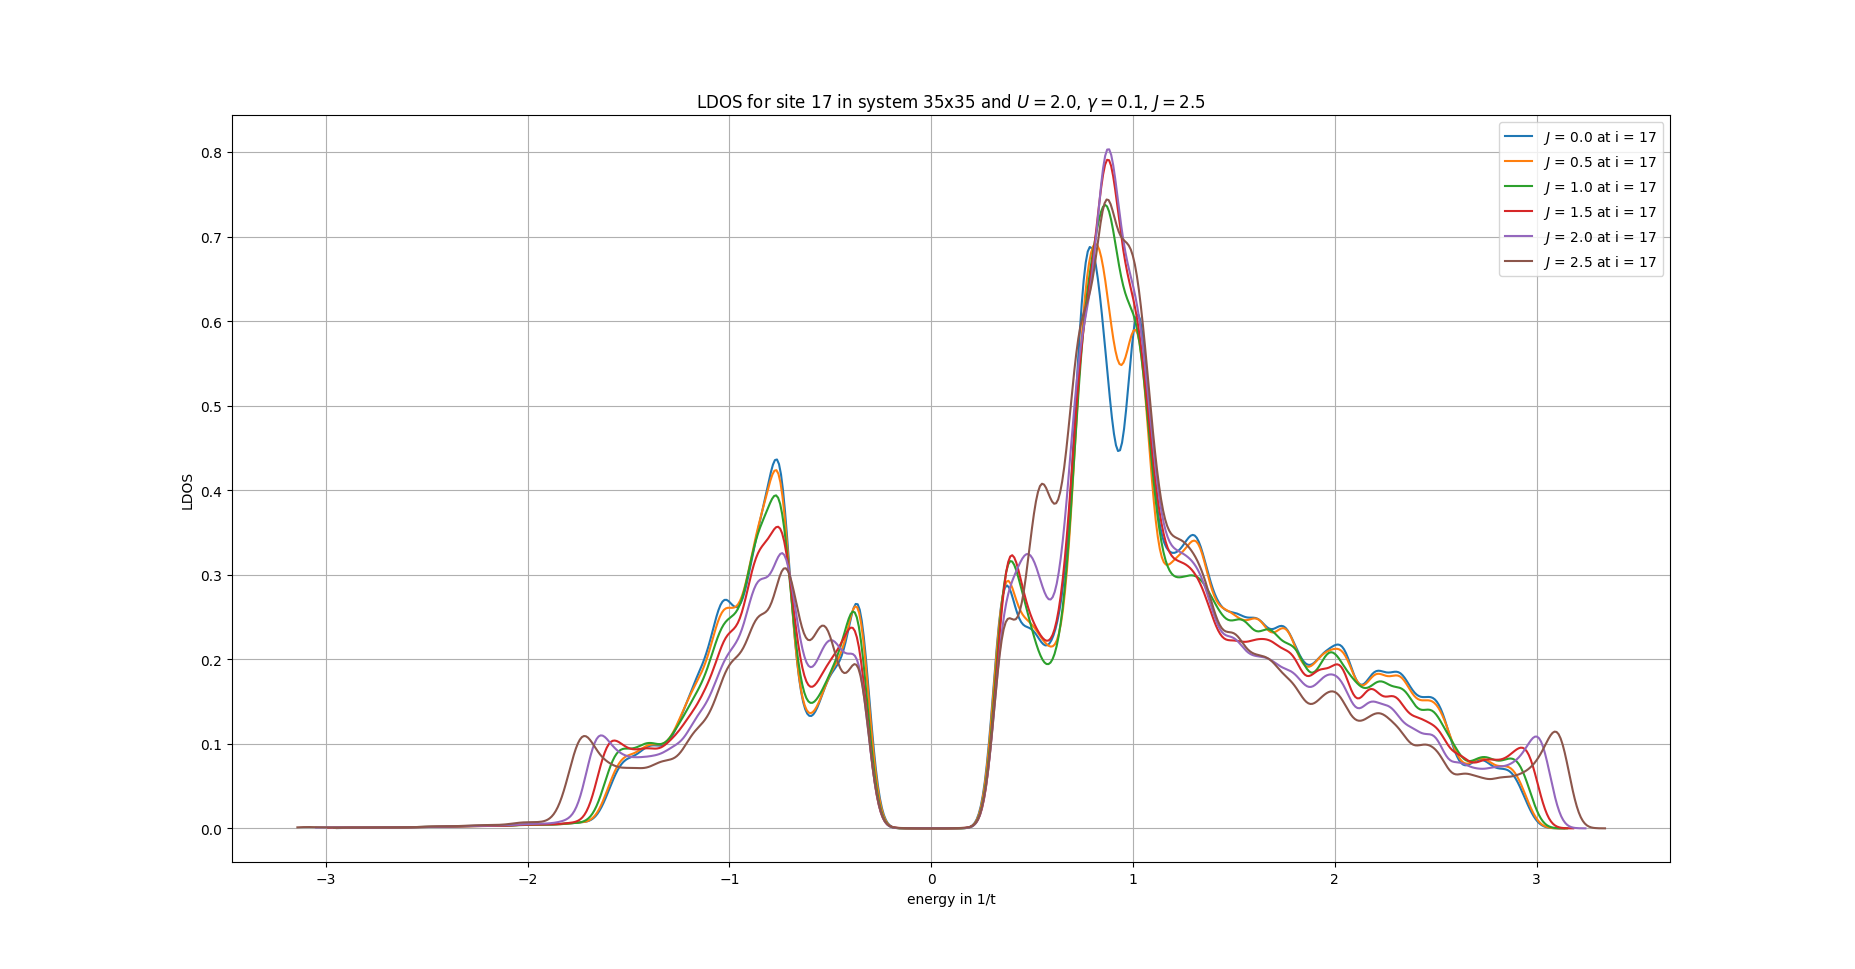
\includegraphics[width=0.95\textwidth]{Images/rkky_35x35_ldos.png}
    \caption{The triplet gap structure becomes less visible for stronger RKKY interaction.}
    \label{fig:ldos_rkky_stronger}
\end{figure}

\subsection{Spin Configuration}
The spin configuration of the impurities is examined by comparing the free energy of the system for different configurations.
In all following plots the labels $\uparrow \,(\downarrow)$ for positive (negative) $S_z$, $\rightarrow \, (\leftarrow)$ for positive (negative) $S_x$ and $x \, (.)$ for positive (negative) $S_y$. \newline
As a validation for the code, the normal metal case with and without SOC is plotted in Figure \ref{fig:spin_normal}.
In both cases, a change in distance leads to oscillatory changes in the spin structure. \newline
It is clearly visible in Figure \ref{fig:spin_normal} (a) that parallel spin configurations in all three directions minimize the free energy, regardless of their sign. 
This is the expected Heisenberg spin-structure. \newline
For a normal metal with SOC, the spin structure becomes component sensitive. 
As expected from the analytical spin structure for this case \cite{valizadeh_mohammad_m_magnetic_2017}, the $S_yS_y$ configuration becomes speical and minimizes the energy for short distances between the two impurities.
For longer distances, the $S_z S_z$ configuration yields the same free energy as the $S_yS_y$ configuration.
\begin{figure}[H]
    \centering
    \label{fig:spin_normal}
    \subfigure[no SOC]{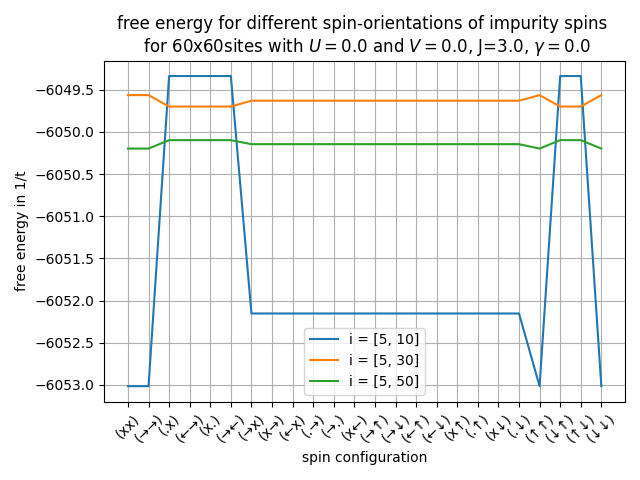
\includegraphics[width=0.48\textwidth]{Images/spinstructure_60_60_0.5_0.0_0.0_0.0_3.0_10_30.png}}
    \subfigure[with SOC]{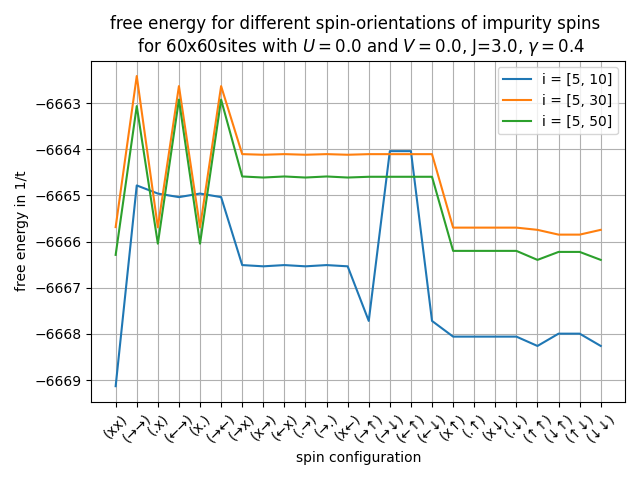
\includegraphics[width=0.48\textwidth]{Images/spinstructure_60_60_0.5_0.0_0.0_0.4_3.0_10_30.png}}
    \caption{Free energy of different spin configurations for a normal metal with two impurity spins. (a) has no SOC, while (b) has $\gamma=0.4$t }
\end{figure}

For the case of a pure singlet pairing superconductor, it is expected that the spin structure changes \cite{SOMEONE SMART} \textcolor{red}{What do I actually expect?}. \newline
Figure \ref{fig:spin_SC} illustrates that a $S_z \neq 0$ rises the free energy significantly. 
Therefore an in-plane spin configuration of the impurity spins is favored for a superconductor. \newline
This preferences does not change with SOC present, but the component sensitivity as in the normal metal case arises.
\textcolor{red}{EXPLANATION}
\begin{figure}[H]
    \centering
    \label{fig:spin_SC}
    \subfigure[no SOC]{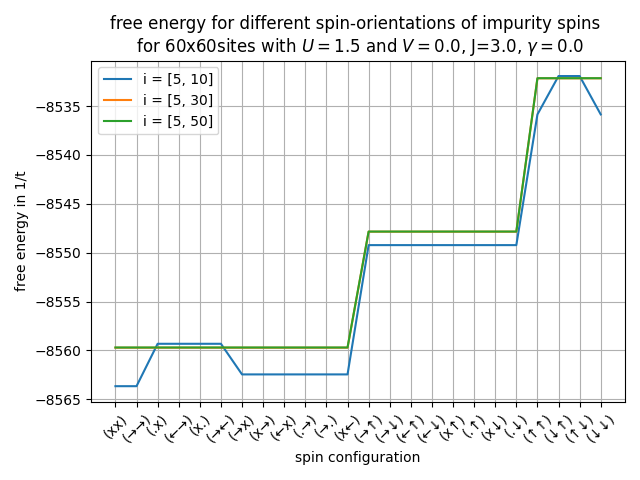
\includegraphics[width=0.48\textwidth]{Images/spinstructure_60_60_0.5_1.5_0.0_0.0_3.0_10_30.png}}
    \subfigure[with SOC]{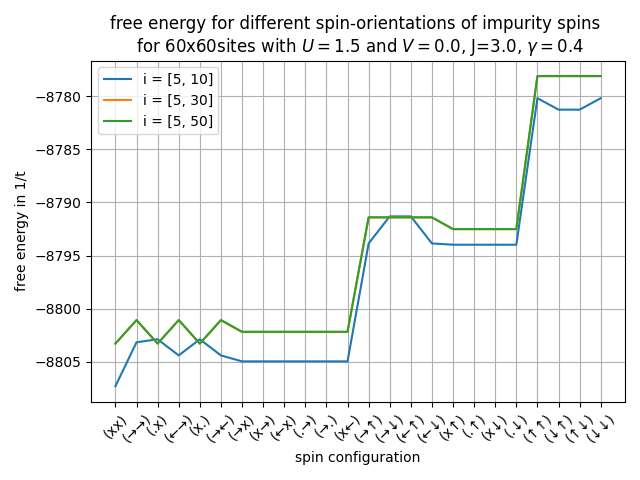
\includegraphics[width=0.48\textwidth]{Images/spinstructure_60_60_0.5_1.5_0.0_0.4_3.0_10_30.png}}
    \caption{Free energy of different spin configurations for a superconductor with two impurity spins. (a) has no SOC, while (b) has $\gamma=0.4$t }
\end{figure}

When triplet pairing is allowed but weaker than the singlet pairing, the spin configuration within the superconductor changes in two ways compared to the purely singlet pairing case.
In Figure \ref{fig:spin_sSC} (a), there is a preference for the $S_yS_y$ configuration visible although no SOC is present in the system. 
For an existing SOC, the preference for the $S_yS_y$ configuration is stronger than for the purely singlet SC case, see Figure \ref{fig:spin_sSC} (b) and \ref{fig:spin_SC}. \newline
Additionally, the free energy of spin configurations containing anti-parallel $S_zS_z$ components is lowered.
It also changes for configurations containing only one $S_z$ component. 
\textcolor{red}{describe more detailed and explain}

\begin{figure}[H]
    \centering
    \label{fig:spin_sSC}
    \subfigure[no SOC]{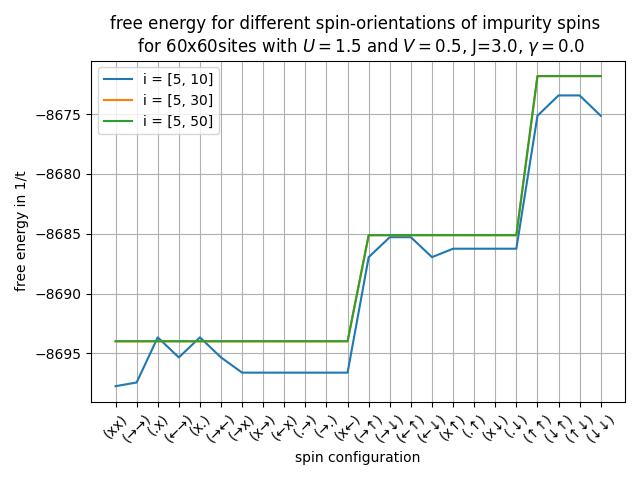
\includegraphics[width=0.48\textwidth]{Images/spinstructure_60_60_0.5_1.5_0.5_0.0_3.0_10_30.png}}
    \subfigure[with SOC]{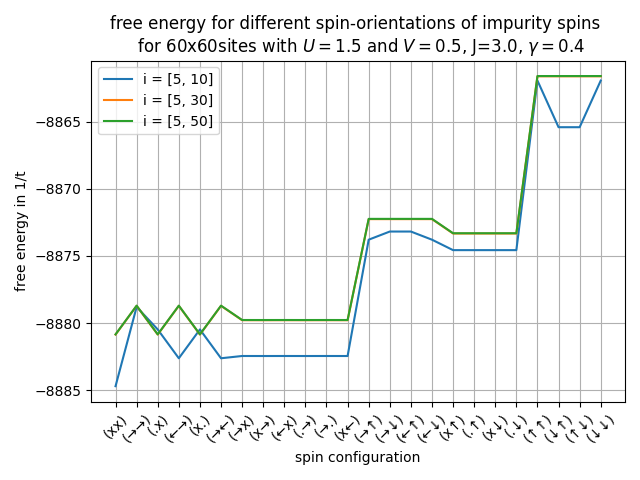
\includegraphics[width=0.48\textwidth]{Images/spinstructure_60_60_0.5_1.5_0.5_0.4_3.0_10_30.png}}
    \caption{Free energy of different spin configurations for a superconductor with two impurity spins, where the singlet pairing is stronger than the triplet pairing. (a) has no SOC, while (b) has $\gamma=0.4$t }
\end{figure}

In a superconductor that is dominated by triplet pairing, the spin structure changes again.
\textcolor{red}{How? Why?}

\begin{figure}[H]
    \centering
    \label{fig:spin_tSC}
    \subfigure[no SOC]{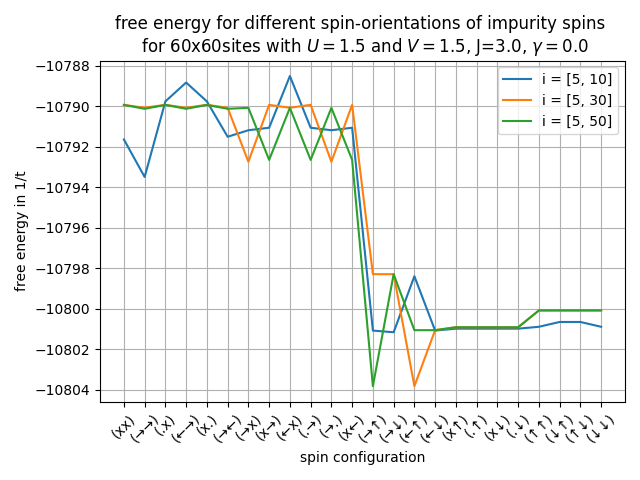
\includegraphics[width=0.48\textwidth]{Images/spinstructure_60_60_0.5_1.5_1.5_0.0_3.0_10_30.png}}
    \subfigure[with SOC]{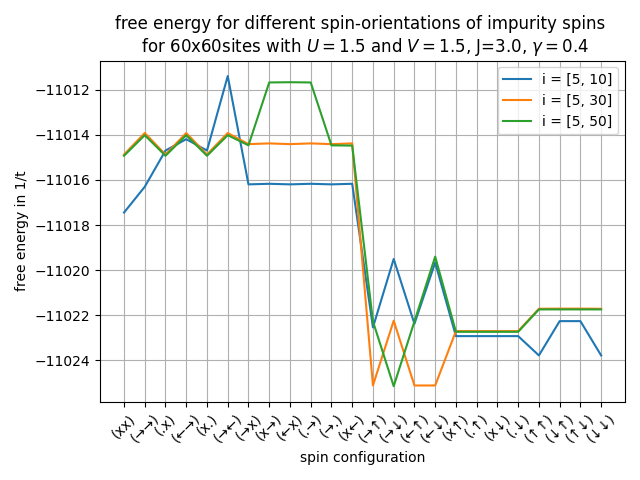
\includegraphics[width=0.48\textwidth]{Images/spinstructure_60_60_0.5_1.5_1.5_0.4_3.0_10_30.png}}
    \caption{Free energy of different spin configurations for a superconductor with two impurity spins, where the triplet pairing is stronger than the singlet pairing. (a) has no SOC, while (b) has $\gamma=0.4$t }
\end{figure}


% \begin{figure}[H]
%     \centering
%     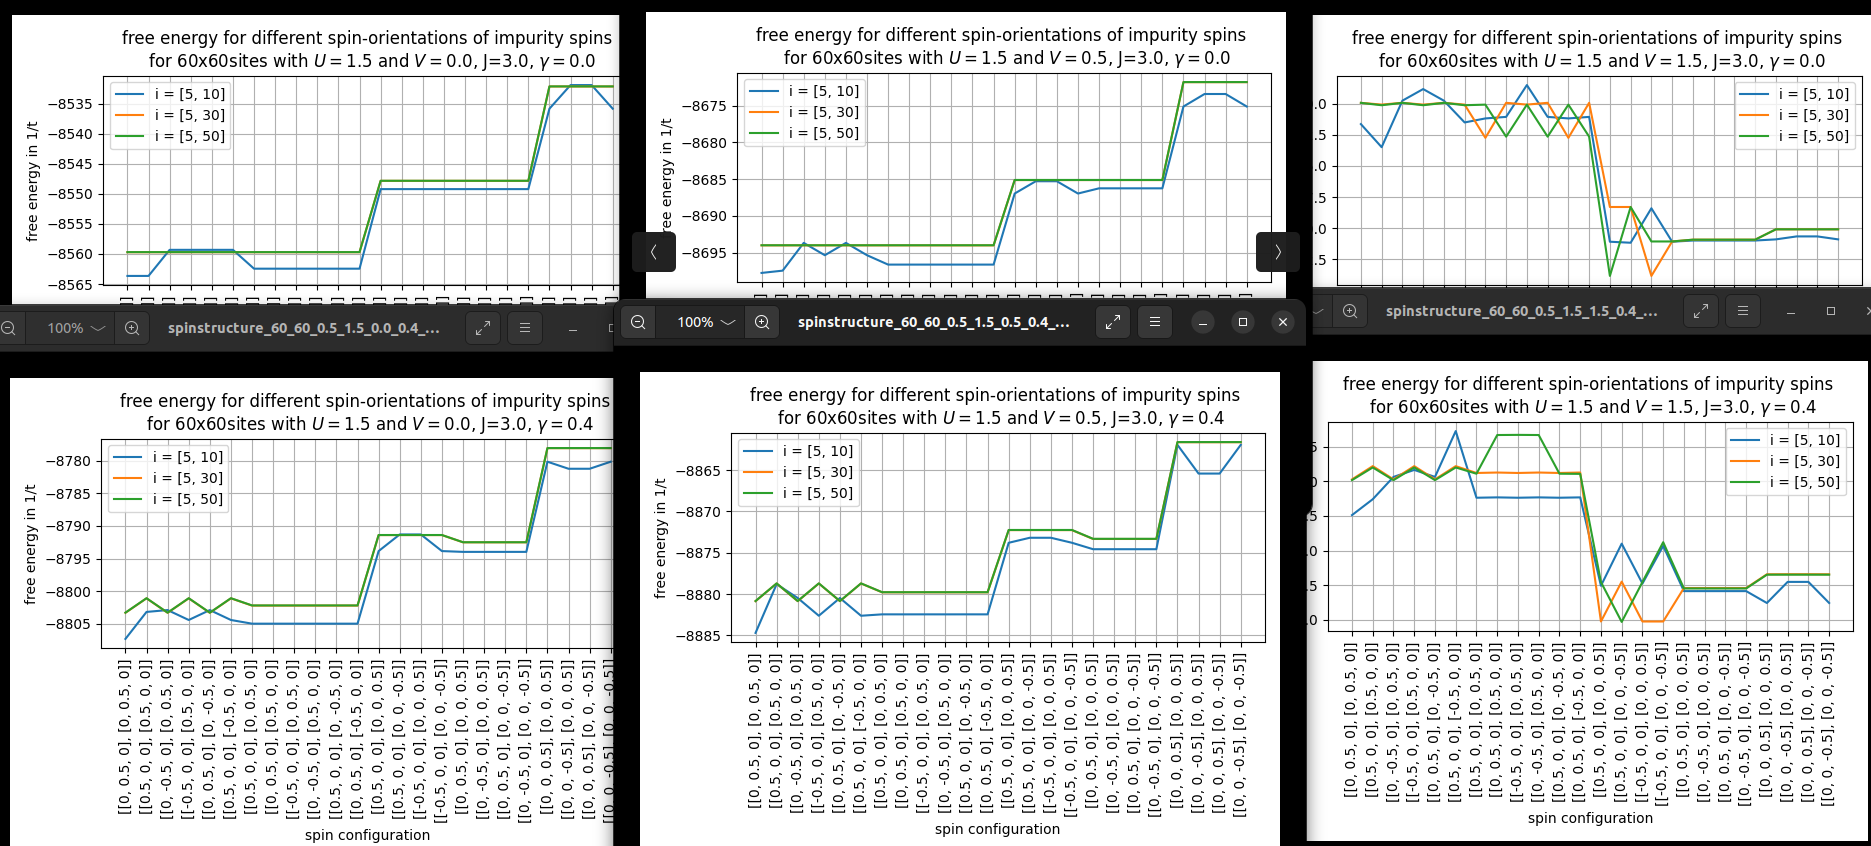
\includegraphics[width=1.2\textwidth, angle=-90]{Images/spinstructure_comp.png}
%     \caption{Spin-structure for different triplet pairing strengths, for $\gamma=0$ (upper graphs) and $\gamma=0.4$ (lower graphs)}
%     \label{fig:free_spin_config_dis}
% \end{figure}

